\chapter{Krabička}
%Základna Jako poslední část jsem potřebovala krabičku – nějakou základnu, která by sjednotila jednotlivé komponenty do jednoho kompletního celku. 
Rozměry krabičky byli designované podle nejrozměrnější komponenty v elektrickém obvodu, což byl držák s bateriemi, jehož rozměry byly 75mm x 42 mm x a na výšku 20mm. Druhou největší komponentou v obvodu byla deska ESP32-DevKitC s rozměry: 55mm x 30 mm x s výškou 10 mm.
Podle výše zmíněných dvou nevětších komponent byly stanoveny přibližné vnitřní rozměry základny: 82 mm x 82 mm x 45 mm, které zaručovali, že se do základny vejde jak ESP32-DevKitC tak baterky, zůstane nějaká rezerva na kabely a další komponenty a základna nebude o moc větší než růže.  
Aby byla ověřena správnost rozměrů, byl podle nich vytvořen první prototyp.
%abych ověřila správnost rozměrů, rozhodla jsem se podle nich vytvořit první prototyp.
%82 mm x 82 mm x 45 mm,



\section{První prototyp}
První prototyp byl vyroben ručně ze 4 mm široké překližky. Podle toho se poté přibližně odvodily vnější rozměry základny. U tohoto prototypu to přibližně bylo: 90 x 90 x 50 mm. Tato práce nebyla profesionální, proto se výsledné rozměry základny nepatrně lišily (+/-2 mm).
%jsem vyrobila ručně

Pro sestavení krabičky bylo z překližky vyřezáno šest dílů: Vrchní a spodní díl 90 x 90mm, a 4 boční stěny o rozměrech 45 x 90 a 45 x 82. Do vrchního dílu se ještě vyřezal kruhový otvor o průměru 28 mm, pro umístění odlité růže a do jednoho bočního dílu vytvořila vrtačkou otvor pro menší přepínací tlačítko. Do rohů byly, přilepeny lepidlem Herkules, špalíčky 10 x 10 mm, které drželi všechny desky základny u sebe a později sloužili pro držení vrchního dílu a růží pomocí šroubků. Takže se vrchní díl s růží mohl kdykoliv sundat a bylo možné manipulovat s Elektrotechnikou uvnitř.

%todo jak je to s přívlastky? 
%Dva čtverce o šířce přibližně 90 mm
%2 obdélníky o výšce 45 mm a délce 90
%2 obdélníky o výšce 45 mm a délce 82
\begin{figure}[htbp]
	\centering
	\begin{minipage}[b]{0.5\textwidth}
		\centering
		\includegraphics[width=0.8\textwidth]{img/06 zakl/Ama základna.jpg}
		\caption{1. prototyp}
		%		\label{fig:gear-sketch1}
	\end{minipage}
	\qquad
	\begin{minipage}[b]{0.4\textwidth}
		\centering
		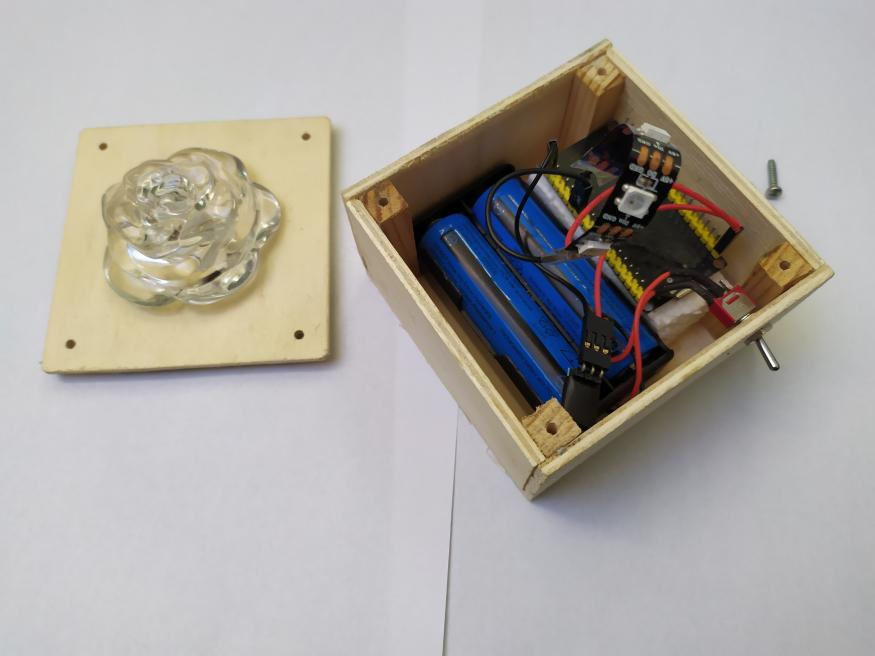
\includegraphics[width=1\textwidth]{img/06 zakl/1. prototyp s ele.jpg}
		\caption{1. prototyp s elektronikou}
		%		\label{fig:gear-sketch2}
	\end{minipage}
\end{figure}

Po sestavení krabičky byl pro kontrolu do krabičky vložen náš elektrický obvod.
Jelikož pokus s prvním prototypem proběhl úspěšně, začalo se pracovat dokonalejším 2 prototypem.


\section{Druhý prototyp základny }
Druhý prototyp základny byl také vyroben ze dřeva, tentokrát ale byly jednotlivé stěny krabice vypáleny na laseru. Díky čemuž prototyp působil profesionálněji. Při této výrobě byla použita překližka široká 3mm. Jednotlivé díly krabičky byli navržené programu zvaný Lightburn.

\subsection{Práce s Lightburnem}
Lightburn je placený editační Software, který škola používá pro práci s Laserovými řezačkami.  Lightburn má speciální funkci na zadávání vnitřních rozměrů základny, takže nebylo třeba počítat vnější rozměry základny a stačilo pouze zadat šířku překližky. Pomocí automatického generátoru, se navíc na okraje komponentů přidali zámky, aby spojování krabičky dohromady bylo jednodušší a nemuseli se použít špalíčky. Jinak zbytek rozměrů zůstal beze změny.

%todo *Obrázek*

\begin{figure}[htbp]
	\centering
	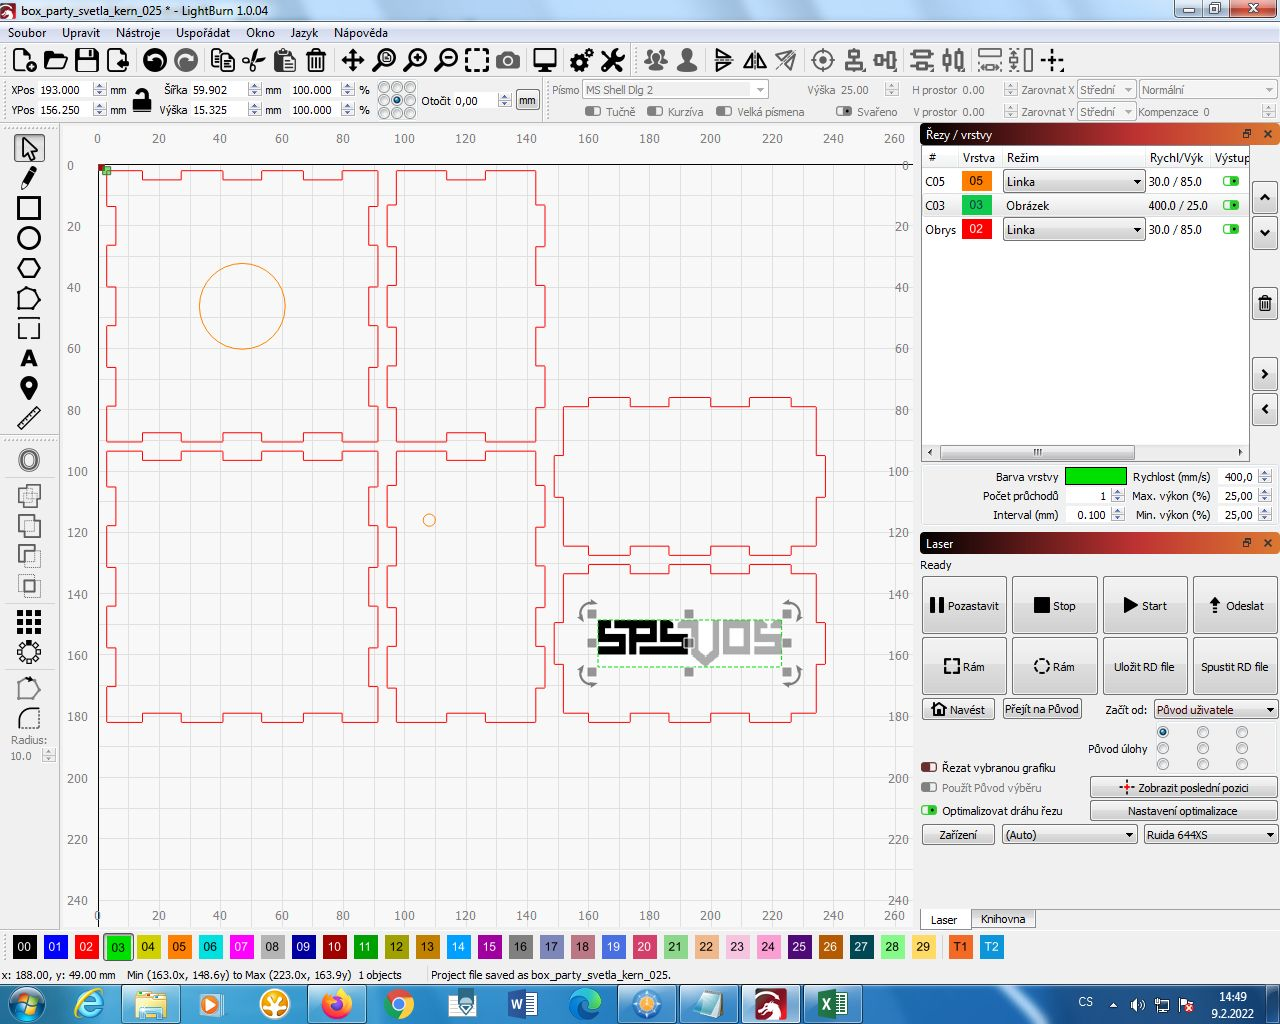
\includegraphics[width=0.5\textwidth]{img/06 zakl/LightBurn_ukazka.jpg}
	\caption{LightBurn}
	%	\label{fig:install-sdk-3}
\end{figure}

Poté stačilo uložit tento soubor ve formátu .slv, nahrát ho do Laserové vypalovačky a z něj vypálit naši krabičku. Výsledek působil reprezentativně, takže se nakonec na laseru vypálili i krabičky pro zbývající prototypy. 


\subsection{Vložení Elektrotechniky a Růže do krabičky}
Krabičky pak byly složeny do své finální podoby a jejich rohy byly zpevněny lepidlem Herkules, aby krabičky lépe držely pohromadě. Jediný kus, který nebyl přilepen, byl vrchní díl s růží, aby se kdykoliv v případě potřeby mohl sundat. 


Poté byl vložen elektrický obvod. Přepínač byl upevněn do otvoru na tlačítko, do základny byl položen opatrně držák s bateriemi a ESP32-DevKitC byl umístěn na kousek polystyrenu, aby v krabičce jen tak neležel a nelítal. 
%Todo lépe zdůvodnit ten polystyren, kabely byli douhé. (nevhodně ustřižené)
Ohebný LED pásek byl opatrně ohnut do obloučku a vložen do otvoru v růži. Poté bylo opatrně přiděláno vrchní víko a bylo hotovo. 
%todo nevím jak to zakončit. 

\begin{figure}[htbp]
	\centering
	\begin{minipage}[b]{0.45\textwidth}
		\centering
		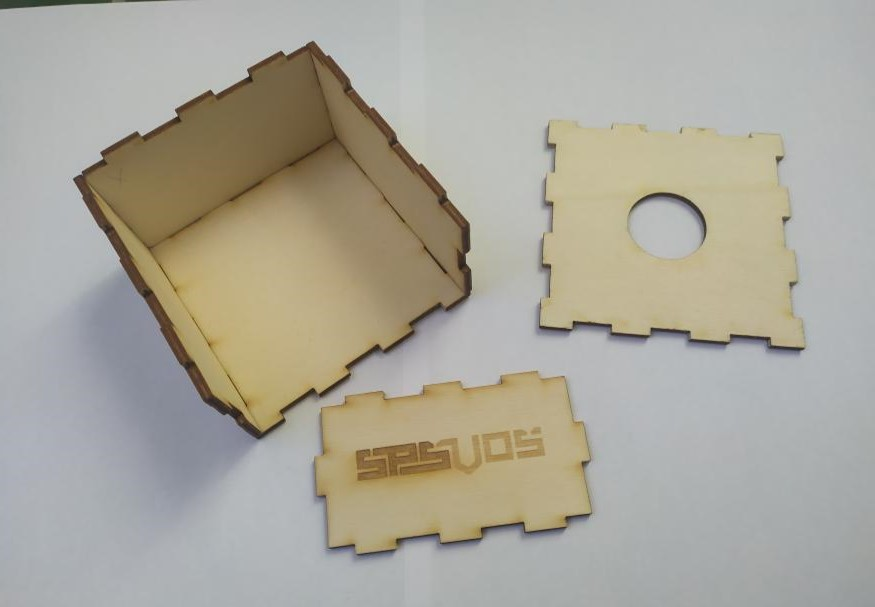
\includegraphics[width=1.1\textwidth]{img/06 zakl/Box.jpg}
		\caption{2. prototyp}
		%		\label{fig:gear-sketch1}
	\end{minipage}
	\qquad
	\begin{minipage}[b]{0.45\textwidth}
		\centering
		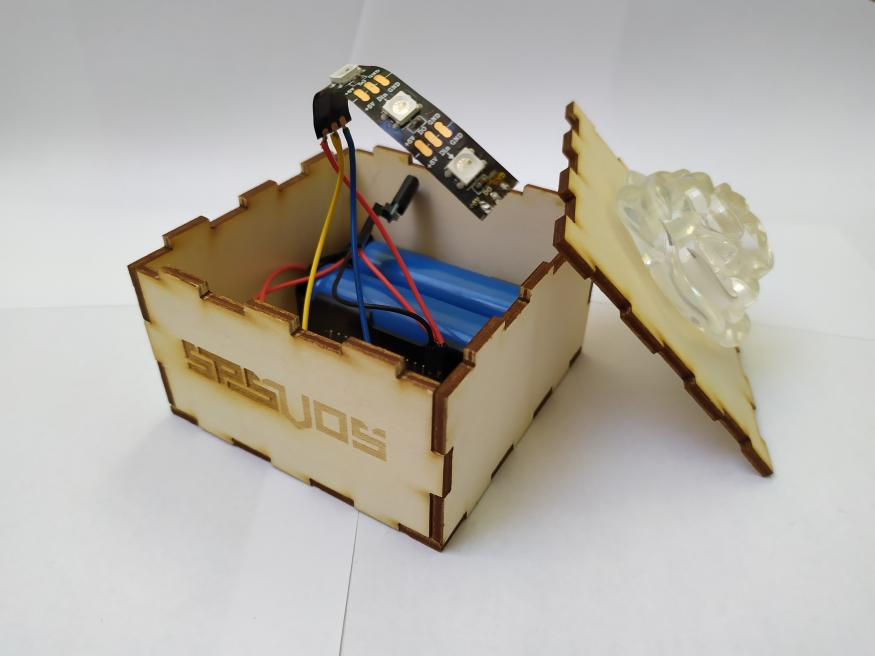
\includegraphics[width=1.01\textwidth]{img/06 zakl/2. prototyp s ele2 .jpg}
		\caption{2. prototyp s elektronikou}
		%		\label{fig:gear-sketch2}
	\end{minipage}
\end{figure}

\newpage
